\documentclass[a4paper,11pt]{article}

\usepackage[a4paper,margin=2.3cm]{geometry}
\usepackage{graphicx}

\title{Stack Layout}
\author{Ruairidh MacGregor}
\date{}

\begin{document}

\maketitle

\section{Layout}

Each TSO contains a data stack, used in exactly the same way as other PLs, e.g. local variables, return addresses and so fourth. The stack grows downwards, with the topmost word pointed to by a local stack pointer.
\newline\newline
The stack consists of a sequence of stack frames, where each frame has the same basic layout of a heap object, e.g. header, payload. There are many types of stack frames, but the most common type are those pushed when evaluating a case expression. To evaluate this expression, it creates a new stack frame which contains the return results from the case statements and continues to evaluate the expression in the case statement, which temporary data for this, would be stored on the stack. Once the thunk has been evaluated, it returns to the previous stack frame and selects the appropriate value that satisfies the case expression.

\section{Info Table}

The info table for a stack frame has a couple extra fields in addition to the basic layout (See heap\_objects.tex). A stack frame info table is defined by \textbf{StgRetInfoTable} in\newline"includes/rts/storage/InfoTables.h".

\begin{figure}
    \centering
    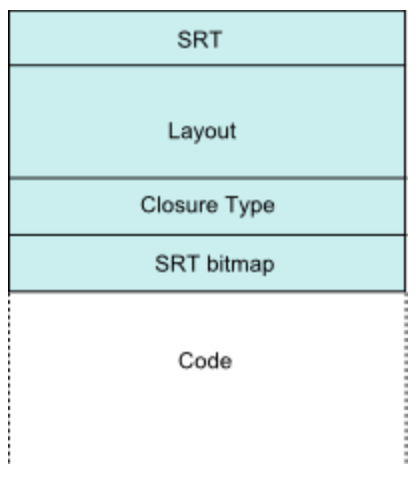
\includegraphics[width=\linewidth]{GHC RTS Notes/Storage/images/stack_info.png}
    \caption{Info table layout for the Stack}
    \label{fig:my_label}
\end{figure}

The SRT field points to the static reference table (SRT) for this stack frame (See CAFs Garbage Collection)

\section{Layout of the Payload}

Unlike heap objects which mainly have "pointers first" layout, in a stack frame the pointers and non-pointers are intermingled.  This is so that we can support "stack stubbing" whereby a live variable stored on the stack can be later marked as dead simply by pushing a new stack frame that identifies that slot as containing a non-pointer, so the GC will not follow it. Therefore, stack frames have the bitmap layout.

\end{document}